\documentclass[12pt]{article}
\usepackage[english,russian]{babel}
\usepackage[left=2cm,right=2cm,top=2cm,bottom=2cm,bindingoffset=0cm]{geometry}
\linespread{1.3}
\usepackage{proof}
\usepackage{amsmath}
\usepackage{amssymb}
\usepackage{graphicx}
\usepackage{stmaryrd}

\title{logic hw theory solutions}
\date{itmo cs t4 2023}
\author{by Petrova Ksenia (cs y2021)}

\begin{document}

\maketitle

\section*{prac 1}

\subsection*{схемы аксиом для КИВ}

(1) & $\alpha \rightarrow \beta \rightarrow \alpha$ \\
(2) & $(\alpha \rightarrow \beta) \rightarrow (\alpha \rightarrow \beta \rightarrow \gamma) \rightarrow (\alpha \rightarrow \gamma)$ \\
(3) & $\alpha \rightarrow \beta \rightarrow \alpha \& \beta$\\
(4) & $\alpha \& \beta \rightarrow \alpha$\\
(5) & $\alpha \& \beta \rightarrow \beta$\\
(6) & $\alpha \rightarrow \alpha \vee \beta$\\
(7) & $\beta \rightarrow \alpha \vee \beta$\\
(8) & $(\alpha \rightarrow \gamma) \rightarrow (\beta \rightarrow \gamma) \rightarrow (\alpha \vee \beta \rightarrow \gamma)$\\
(9) & $(\alpha \rightarrow \beta) \rightarrow (\alpha \rightarrow \neg \beta) \rightarrow \neg \alpha$\\
(10) & $\neg \neg \alpha \rightarrow \alpha$

\subsection*{task 3g}

task: $\vdash ((A \rightarrow B) \rightarrow A)\rightarrow A$ (закон Пирса)\\
по теореме о дедукции достаточно доказать: $(A \rightarrow B) \rightarrow A \vdash A$

\begin{enumerate}
    \item $(\phi \rightarrow \pi) \rightarrow (\psi \rightarrow \pi) \rightarrow (\phi \vee \psi \rightarrow \pi)$ - аксиома 8\\
    $\phi = A \rightarrow B\quad
    \pi = A\quad
    \psi = A$\\
    $((A \rightarrow B) \rightarrow A) \rightarrow (A \rightarrow A) \rightarrow ((A \rightarrow B) \vee A \rightarrow A)$
    \item $\infer{(A \rightarrow A) \rightarrow ((A \rightarrow B) \vee A \rightarrow A)}
    {(A \rightarrow B) \rightarrow A \quad ((A \rightarrow B) \rightarrow A) \rightarrow (A \rightarrow A) \rightarrow ((A \rightarrow B) \vee A \rightarrow A)}$
    \item ранее доказано: $A \rightarrow A$
    \item $\infer{(A \rightarrow B) \vee A \rightarrow A}
    {A \rightarrow A\quad (A \rightarrow A) \rightarrow ((A \rightarrow B) \vee A \rightarrow A)}$
    \item гипотеза: $(A \rightarrow B) \rightarrow A\quad\Rightarrow \quad
    A \rightarrow B \vdash A \quad \Rightarrow \quad A \rightarrow B$
    \item $\alpha \rightarrow \alpha \vee \beta$ - аксиома 6\\
    $\alpha = A \rightarrow B\quad \beta = A$\\
    $(A \rightarrow B) \rightarrow (A \rightarrow B) \vee A$
    \item $\infer{(A \rightarrow B) \vee A}
    {A \rightarrow B\quad (A \rightarrow B) \rightarrow (A \rightarrow B) \vee A}\quad$ (5, 6 пункты)
    \item $\infer{A}
    {(A \rightarrow B) \vee A\quad (A \rightarrow B) \vee A \rightarrow A}\quad$ (4, 7 пункты)
\end{enumerate}

\section*{prac 3}
\subsection*{определения}

\emph{Замкнутое} множество --- такое, дополнение которого открыто.\\
\emph{Внутренностью} множества $A^\circ$ назовём наибольшее открытое множество, содержащееся в $A$.\\
\emph{Замыканием} множества $\overline{A}$ назовём наименьшее замкнутое множество, содержащее $A$.\\
Назовём \emph{окрестностью} точки $x$ такое открытое множество $V$, что $x \in V$.\\
Будем говорить, что точка $x \in A$ \emph{внутренняя}, если существует окрестность $V$, что $V \subseteq A$.\\
Точка $x$ --- \emph{граничная}, если любая её окрестность $V$ пересекается как с $A$, так и с его дополнением.


\subsection*{task 1a}

task: покажите, что $A$ открыто тогда и только тогда, когда все точки $A$ --- внутренние.
Также покажите, что $A^\circ = \{ x\ |\ x \in A\ \&\ x$ --- внутренняя точка$\}$.

\textbf{proof:}\\
$\Rightarrow\quad$
$A$ --- открытое $ \Rightarrow \forall x\ |\ x \in A\ \exists\ V_x = A$ --- открытое и $A \subseteq A \Rightarrow x$ --- внутренняя\\
$\Leftarrow\quad$ $\forall x \in A\ \exists\ V_x\ |\ V_x \in A\ \&\ V_x$ --- открытое\\
$V_x$ --- открытое $\Rightarrow V_x \in \Omega$\\
Возьмём $V_x\ \forall x \in A \Rightarrow \bigcup_{x \in A} V_x \in \Omega$\\
$\bigcup_{x \in A} V_x = A \Rightarrow A \in \Omega \Rightarrow A$ --- открытое\\

\textbf{proof:}\\
$A^\circ$ --- наибольшее открытое множество $|\ A^\circ \subseteq A$\\
Рассмотрим $A^\circ \cup x\ |\ x \notin A$\\
$\left[ 
    \begin{gathered}
    A^\circ \cup x \textrm{ --- не открытое} \Rightarrow x \textrm{ --- не внутренняя}
    \\
    A^\circ \cup x \nsubseteq A \Rightarrow x \notin A
    \end{gathered}
\right.$
$\qquad\Rightarrow \forall x\ |\ x \in A^\circ \Rightarrow x \in A\ \&\ x$ --- внутренняя

\subsection*{task 1b}

task: покажите, что $A$ замкнуто тогда и только когда, когда содержит все свои граничные точки. Также покажите, что $\overline{A} = \{ x\ |\ x\text{ --- внутренняя или граничная точка}\}$. Верно ли, что $\overline{A} = X \setminus ((X\setminus A)^\circ)$?

\textbf{proof:}\\
$\Rightarrow\quad $
Пусть $\exists\ x$ --- граничная точка для $A\ |\ x \notin A \Rightarrow x \in A^c$\\
$A$ --- замкнутое $\Rightarrow A^c$ --- открытое $\Rightarrow x$ --- внутренняя для $A^c \Rightarrow\\
\exists\ V_x\ |\ V_x \subseteq A^c\Rightarrow V_x \cap A = \varnothing \Rightarrow x$ --- не граничная для $A \Rightarrow$\\
любая граничная для $A$ точка принадлежит $A$\\
$\Leftarrow\quad$
$A$ содержит все свои граничные точки $\Rightarrow$ не все точки $A$ внутренние $\Rightarrow\\
A$ --- не открытое $\Rightarrow A$ --- замкнутое\\ \\
task: Также покажите, что $\overline{A} = \{ x\ |\ x\text{ --- внутренняя или граничная точка}\}$.

\textbf{proof:}\\
Рассмотрим $x$ - внутренняя для $A$ и $x \notin \overline{A}$\\
$x$ - внутренняя для $A \Rightarrow x \in A$ и $x \notin \overline{A} \Rightarrow A \nsubseteq \overline{A} \Rightarrow \overline{A}$ --- не замыкание $A$\\ \\
Рассмотрим $x$ - граничная для $A$ и $x \notin \overline{A}$\\
$x$ - граничная для $A \Rightarrow \exists\ V_x\ |\ V_x \cap A \neq \varnothing$\\
$A \subseteq \overline{A} \Rightarrow V_x \cap \overline{A} \neq \varnothing \Rightarrow x$ --- граничная для $\overline{A}$ или $x$ --- внутренняя для $\overline{A}$\\
Если $x$ --- граничная для $\overline{A}$ и $x \notin \overline{A} \Rightarrow \overline{A}$ --- не замкнутое\\
Если $x$ --- внутренняя для $\overline{A}$ и $x \notin \overline{A} \Rightarrow x$ --- не внутренняя для $\overline{A}$\\\\
% Покажем, что в $\overline{A}$ не может быть внутренних точек для $A^c$\\\\
task: Верно ли, что $\overline{A} = X \setminus ((X\setminus A)^\circ)$?

\textbf{proof:}\\
$X \setminus A = A^c$\\
$(X\setminus A)^\circ = (A^c)^\circ = A^c \setminus \partial A$\\
$X \setminus ((X\setminus A)^\circ) = X \setminus (A^c)^\circ = X \setminus (A^c \setminus \partial A) = A \cup \partial A = \overline{A}$

% \section*{task 1d}

% task: Пусть $A \subseteq B$. Как связаны $A^\circ$ и $B^\circ$, а также $\overline{A}$ и $\overline{B}$?

% покажем, что $A^\circ \subseteq B^\circ$\\
% \textbf{proof:}\\
% рассмотрим $x \in A^\circ \Rightarrow \exists V_x\ |\ V_x \subseteq A$

\subsection*{task 1f}

task: Покажите, что $\overline{\left(\overline{A^\circ}\right)^\circ} = \overline{A^\circ}$.\\

\textbf{proof:}\\
Пусть $B = \overline{A^\circ}$. Заметим, что $B$ --- замкнутое множество, значит содержит все свои граничные точки\\
$B^\circ = B \setminus \partial B$\\
$\overline{B^\circ} = (B \setminus \partial B) \cup \partial B = B$

\subsection*{task 2a}

task: Связны ли $\mathbb{Q}$ и $\mathbb{R}\setminus\mathbb{Q}$ как топологические подпространства $\mathbb{R}$?\\
$A \subseteq X$ --- несвязное как подпространство $\mathbb{R}$, если $\exists\ U, V \subseteq X\ |\ U, V \in \Omega$ и удовлетворяют условиям:
\begin{enumerate}
    \item $U\cap A \neq \varnothing,\ V\cap A \neq \varnothing$
    \item $U \cap V \cap A = \varnothing$
    \item $A \subseteq U \cup V$
\end{enumerate}

\textbf{proof:}\\
Рассмотрим $A = \bigcup_{n = 0}^{\infty}(\sqrt{2} + n, \sqrt{2} + n + 1)$\\
$B = \bigcup_{n = 0}^{\infty}(\sqrt{2} - n - 1, \sqrt{2} - n)$\\
$A, B \in \Omega$ как счётное объединение открытых на $\mathbb{R}$ множеств
\begin{enumerate}
    \item $A\cap \mathbb{Q} \neq \varnothing,\ B\cap \mathbb{Q} \neq \varnothing$
    \item $A \cap B \cap \mathbb{Q} = \varnothing$
    \item $\mathbb{Q} \subseteq A \cup B$
\end{enumerate}
$\mathbb{Q}$ - несвязное как подпространство\\
С $\mathbb{I} = \mathbb{R} \setminus \mathbb{Q}$ аналогично, только 0 вместо $\sqrt{2}$
\begin{figure}[h!]
    \centering
    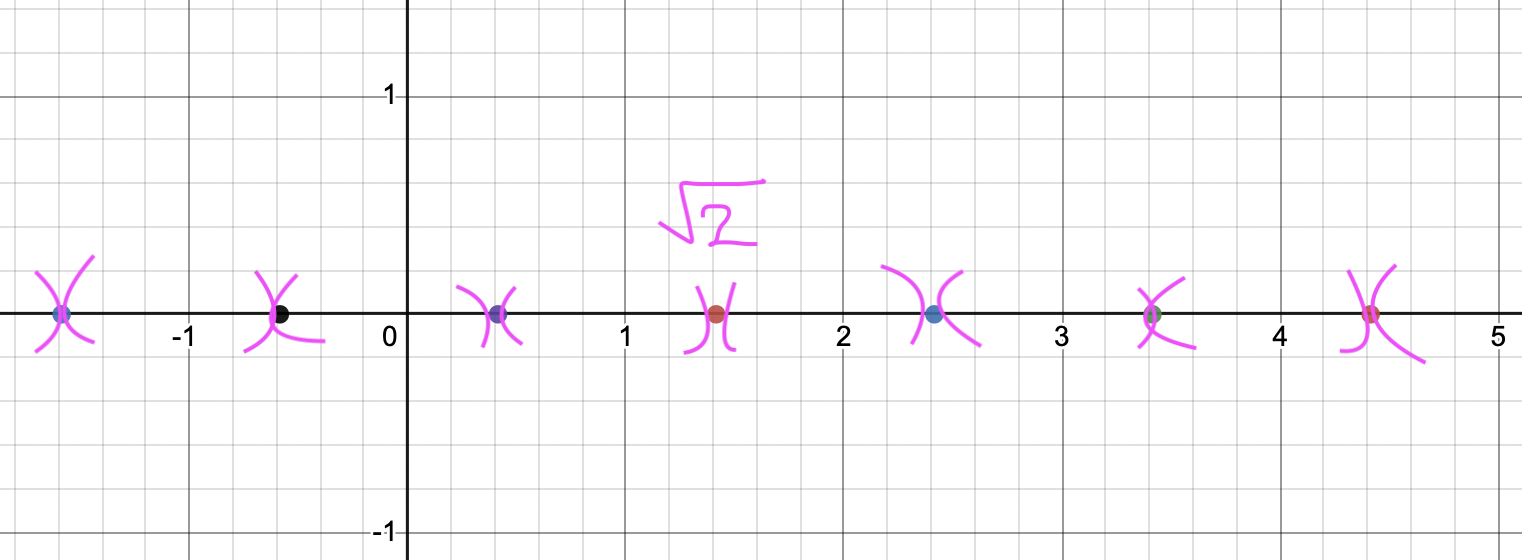
\includegraphics[width=1\linewidth]{hehe.png}
    \label{2}
\end{figure}

\subsection*{task 2b}

покажем, что $\nexists\ A, B \in \Omega\ |\ A\cup B = (0,1),\ A\cap B = \varnothing,\ A, B \neq \varnothing$\\
попробуем найти $A =(a_0,a_1),\ B =(b_0,b_1)$, удовлетворяющие условиям\\
$(a_0,a_1)\cup(b_0,b_1) = (0,1)\Rightarrow a_0=0,\ b_1=1$\\
$\left[ 
    \begin{gathered}
    a_1=b_0 \textrm{ или } a_0 > b_1\Rightarrow A\cap B \neq \varnothing
    \\
    a_1 < b_0 \Rightarrow (a_0,a_1)\cup(b_0,b_1) \neq (0,1)
    \\
    \end{gathered}
\right.$

\subsection*{task 3a}

Для каждого из примеров ниже проверьте, задано ли в нём топологическое пространство, и ответьте на следующие вопросы, если это так:
каковы окрестности точек в данной топологии;
каковы замкнутые множества в данной топологии;
связно ли данное пространство.\\

Топология Зарисского на $\mathbb{R}$: 
$\Omega = \{\varnothing\} \cup \{ X \subseteq \mathbb{R}\ |\ \mathbb{R} \setminus X\ \text{конечно} \}$,
то есть пустое множество и все множества с конечным дополнением.

\begin{enumerate}
    \item $\varnothing \in \Omega\quad \mathbb{R}\setminus \mathbb{R} = \varnothing$ --- конечное $\Rightarrow \mathbb{R}\in \Omega$
    \item Пусть $A_i \in \Omega\quad$ $\mathbb{R} \setminus \bigcap_{i=1}^n A_i = \bigcup_{i=1}^n (\mathbb{R}\setminus A_i)$ - конечно, как конечное объединение конечных множеств $\Rightarrow \bigcap_{i=1}^n A_i \in \Omega$
    \item Пусть $A_i \in \Omega\quad$ $\mathbb{R} \setminus \bigcup_{i=1}^\infty A_i = \bigcap_{i=1}^\infty (\mathbb{R}\setminus A_i)$ - конечно, как счётное пересечение конечных множеств $\Rightarrow \bigcup_{i=1}^\infty A_i \in \Omega$
\end{enumerate}
Окрестность точки $x$ --- такое открытое множество $V_x$, что $x \in V_x$\\
Для $x \in A \in \Omega\Rightarrow V_x = A$ --- набор интервалов\\\\
Замкнутые множества - множества, дополнения которых открыты\\
Замкнутые множества: конечные множества (наборы точек)\\\\
Покажем, что $\nexists\ A, B \in \Omega\ |\ A\cup B = \mathbb{R},\ A\cap B = \varnothing,\ A, B \neq \varnothing$\\
Пусть $A \in \Omega \Rightarrow A$ --- набор интервалов. Пусть $ A\cup B = \mathbb{R} \Rightarrow \mathbb{R} \setminus A = B$ --- конечный набор точек $\Rightarrow B \notin \Omega \Rightarrow$ пространство связное

\section*{prac 4}

\subsection*{task 5}

\quad\ task: Покажите аналог теоремы о дедукции для естественного вывода: $\Gamma,\alpha\vdash\beta$ тогда и только тогда, когда
$\Gamma\vdash\alpha\rightarrow\beta$\\

solution

$\Leftarrow$\\
пусть $\Gamma\vdash\alpha\rightarrow\beta$, покажем $\Gamma,\alpha\vdash\beta$
\begin{enumerate}
    \item по условию существует вывод $\infer{\alpha\rightarrow\beta}{\delta_1, \delta_2, \dots, \delta_{n-1}}$
    
    \item $\Rightarrow \infer{\beta}{\delta_1, \delta_2, \dots, \delta_{n-1}, \alpha\rightarrow\beta, \alpha}$ - тоже вывод

    \item в предыдущем пункте $\alpha$ стало гипотезой, а $\beta$ получилось по правилу Modus Ponens из $\alpha\rightarrow\beta$ и $\beta$

    \item $\Rightarrow \Gamma,\alpha\vdash\beta$
\end{enumerate}

$\Rightarrow$\\

воспользуемся правилом введения связок с лекции: $\infer{\Gamma\vdash\alpha\rightarrow\beta}{\Gamma,\alpha\vdash\beta}$

\section*{prac 5}

\subsection*{task 5.6a}

\quad\ task: Покажите, что исчисление предикатов не полно в моделях ограниченной конечной мощности. 
А именно, пусть дана модель $\mathcal{M} = \langle D, F, T, E \rangle$. 
Назовём мощностью модели мощность её предметного множества: $|\mathcal{M}| = |D|$.
Покажите, что для любой конечной мощности модели $n\in\mathbb{N}$ найдётся такая формула $\alpha$, что 
при $|\mathcal{M}|\le n$ выполнено $\llbracket\alpha\rrbracket_\mathcal{M} = \text{И}$, но $\not\vdash\alpha$.\\

solution

\begin{enumerate}
    \item $|D|=n$ - конечная мощность
    
    \item введём в модель операцию равенства $x_1=x_2$, будем оценивать её так: $\llbracket x_1=x_2 \rrbracket=$ И, если $x_1=x_2$
    
    \item рассмотрим формулу $\alpha_k=\exists x_1...x_k.
\bigwedge_{1\leq p < q \leq k}\neg(x_p=x_q)\\
=\exists x_1...x_k.(
\neg(x_1=x_2)\wedge\neg(x_1=x_3)\wedge...\wedge\neg(x_1=x_k)\wedge\neg(x_2=x_3)\wedge...\wedge\neg(x_{k-1}=x_k))$

    \item из лекции знаем, что оценка предметной области $E(x)\ |\ E\subseteq D$. пусть $|E|=|D|=n$ (максимальная можность $|E|$). буквами $a_1...a_n\in D$ будем обозначать значения функции оценки предметных переменных

    \item чтобы большая конъюкция оценивалась в истину, нужно, чтобы каждое равенство оценивалось в ложь $\Rightarrow$ каждую переменную нужно оценить разным элементом из $E\Rightarrow \llbracket x_i \rrbracket = a_i$
    
    \item для любого $k\leq n$ выполнено $\llbracket\alpha_k\rrbracket=$ И, однако для $k=n+1$ так оценить уже не получится и большая конъюкция оценится в ложь ($\llbracket\alpha_{n+1}\rrbracket=$ Л) $\Rightarrow$ формула $\alpha$ не общезначима ($\not\models \alpha$)

    \item теорема о корректности исчисления предикатов: всякая формула, выводимая в классическом исчислении предикатов, общезначима ($\vdash \alpha \Rightarrow\ \models \alpha $)

    $\Rightarrow$ $\not\models \alpha \Rightarrow\ \not\vdash \alpha$ (вспоминаем правило $A\Rightarrow B$ значит $\neg B \Rightarrow \neg A$)

    \item итак, получили, что формула $\alpha_k$ оценивается в истину $\forall k \le n$, но $\not\vdash \alpha$

    \item для общезначимости $\alpha$ и доказемости необходимо, чтобы $|D|=\infty$

\end{enumerate}




\subsection*{task 5.4a}

\quad\ task: Докажите или опровергните (каждую формулу в отдельности): $(\forall x.\exists y.\phi) \rightarrow (\exists x.\forall y.\phi)$ и
$(\exists x.\forall y.\phi) \rightarrow (\forall x.\exists y.\phi)$\\

solution

формула 1: $(\forall x.\exists y.\phi) \rightarrow (\exists x.\forall y.\phi)$

опровергнем:\\
пусть $D=\mathbb{R},\quad \varphi(x,y) = x + y > 0$\\
$\llbracket \forall x.\exists y.\phi \rrbracket=$ И, но $\llbracket \exists x.\forall y.\phi \rrbracket=$ Л

формула 2: $(\exists x.\forall y.\phi) \rightarrow (\forall x.\exists y.\phi)$

опровергнем: $D=\mathbb{R},\quad \varphi(x) = x > 0$\\
$\llbracket \exists x.\forall y.\phi \rrbracket=$ И, но $\llbracket \forall x.\exists y.\phi \rrbracket=$ Л

\section*{prac 6}

\subsection*{task 6.4b}

\quad\ task: Пусть $M$ --- непротиворечивое множество формул и $\mathcal{M}$ --- построенная в соответствии с теоремой о 
полноте исчисления предикатов оценка для $M$. Мы ожидаем, что $\mathcal{M}$ будет моделью для $M$, для чего было необходимо доказать
несколько утверждений. Восполните некоторые пробелы в том доказательстве. А именно, если $\varphi$ --- 
некоторая формула и для любой формулы $\zeta$, более короткой, чем $\varphi$, выполнено
$\mathcal{M}\models\zeta$ тогда и только тогда, когда $\zeta\in M$, тогда покажите:\\
(b) если $\varphi = \neg\alpha$, $\mathcal{M}\models\neg\alpha$, то $\neg\alpha\in M$; и если $\mathcal{M}\not\models\neg\alpha$, то $\neg\alpha\notin M$.\\

solution

\begin{enumerate}
    \item докажем, что если $\varphi = \neg\alpha$, $\mathcal{M}\models\neg\alpha$, то $\neg\alpha\in M$

    \begin{enumerate}
        \item по условию $\mathcal{M}\models\neg\alpha \Rightarrow \llbracket \neg\alpha \rrbracket_\mathcal{M}=$ И $\Rightarrow \llbracket \alpha \rrbracket_\mathcal{M}=$ Л
        \item $\mathcal{M}\not\models\alpha$ и $\alpha$ короче, чем $\neg\alpha\Rightarrow$ по условию $\alpha\not\in M \Rightarrow$ по теореме о полноте $\neg\alpha\in M$
    \end{enumerate}

    \item докажем, что если $\mathcal{M}\not\models\neg\alpha$, то $\neg\alpha\notin M$

    \begin{enumerate}
        \item $\mathcal{M}\not\models\neg\alpha \Rightarrow\llbracket \neg\alpha \rrbracket_\mathcal{M}=$ Л $\Rightarrow \llbracket \alpha \rrbracket_\mathcal{M}=$ И
        \item $\mathcal{M}\models\alpha$ и $\alpha$ короче, чем $\neg\alpha\Rightarrow$ по условию $\alpha\in M \Rightarrow M\vdash \alpha$
        \item предположим, что $\neg\alpha\in M  \Rightarrow M\vdash \neg\alpha$
        \item $M\vdash \alpha$ и $M\vdash \neg\alpha\Rightarrow M$ --- противоречиво, что противоречит условию, значит предположение неверно $\Rightarrow \neg\alpha\not\in M$
    \end{enumerate}

\end{enumerate}

\subsection*{task 6.2a}

\quad\ task: Покажите, что если классическое исчисление высказываний противоречиво, то также противоречиво и интуиционистское исчисление высказываний.\\

solution

предположим, что КИВ противоречиво, то есть $\exists\alpha\ |\ \vdash\alpha\&\neg\alpha$

высказывание $\alpha$ в КИВ эквивалентно высказыванию $\alpha\rightarrow \bot$ в ИИВ

\begin{enumerate}
    \item $\alpha \& \beta \rightarrow \alpha$ --- аксиома 4\\
    $\beta = \neg\alpha$\\
    $\alpha \& \neg\alpha \rightarrow \alpha$
    \item $\infer{\alpha}{\alpha \& \neg\alpha\quad\alpha \& \neg\alpha \rightarrow \alpha}$ --- M.P. предположение и п.1
    \item $\vdash\alpha\Rightarrow\models\alpha$ по теореме о полноте
    \item при любой оценке $\llbracket \alpha \rrbracket$ = И $\Rightarrow \llbracket \alpha \rightarrow \bot \rrbracket$ = Л
    \item $\alpha \& \beta \rightarrow \beta$ --- аксиома 5\\
    $\beta = \neg\alpha$\\
    $\alpha \& \neg\alpha \rightarrow \neg\alpha$
    \item $\infer{\neg\alpha}{\alpha \& \neg\alpha\quad\alpha \& \neg\alpha \rightarrow \neg\alpha}$ --- M.P. предположение и п.5
    \item $\vdash\neg\alpha\Rightarrow\models\neg\alpha$ по теореме о полноте
    \item при любой оценке $\llbracket \neg\alpha \rrbracket$ = И $\Rightarrow \llbracket \alpha \rrbracket$ = Л $\Rightarrow  \llbracket \alpha \rightarrow \bot \rrbracket$ = И
    
\end{enumerate}

пришли к противоречию

\section*{prac 7}

\subsection*{task 7.2e}

task: Определим отношение <<меньше или равно>> так: $0 \le a$ и $a' \le b'$, если $a \le b$. Докажите, что:\\
Будем говорить, что $a$ делится на $b$ с остатком, если существуют такие $p$ и $q$, что 
$a = b \cdot p + q$ и $0 \le q < b$. Покажите, что $p$ и $q$ всегда существуют и единственны,
если $b > 0$.\\

solution\\

$\exists$
\begin{verbatim}
    p = 0
    q = 0 
    while b * p' <= a:
        p = p'
    while b * p + q' <= a:
        q = q'
\end{verbatim}

$\exists !$
\begin{enumerate}
    \item докажем от противного: пусть $\exists p_1, p_2, q_1, q_2\ |\ p_1\neq p_2,\quad q_1\neq q_2,\quad a = b \cdot p_1 + q_1,\\ a = b \cdot p_2 + q_2$
    \item $a = b \cdot p_1 + q_1$ и $b \cdot p_1'>a$ (по тому, как работает алгоритм) $\Rightarrow p_2 \leq p_1$\\
    $p_2\neq p_1\Rightarrow p_2 < p_1$
    \item $a = b \cdot p_2 + q_2$ и $b \cdot p_2'>a$ (по тому, как работает алгоритм) $\Rightarrow p_1 \leq p_2$\\
    $p_1\neq p_2\Rightarrow p_1 < p_2$
    \item противоречие: $p_1=p_2=p$
    \item $a = b \cdot p + q_2$ и $b \cdot p + q_2'>a$ (по тому, как работает алгоритм) $\Rightarrow q_1 \leq q_2$\\
    $q_1\neq q_2\Rightarrow q_1 < q_2$
    \item $a = b \cdot p + q_1$ и $b \cdot p + q_1'>a$ (по тому, как работает алгоритм) $\Rightarrow q_2 \leq q_1$\\
    $q_2\neq q_1\Rightarrow q_2 < q_1$
\end{enumerate}

\subsection*{task 7.3d}

task: Определим <<ограниченное вычитание>>: $$a \dotminus b = \left\{\begin{array}{ll}0, & a = 0\\a, & b = 0\\p \dotminus q, & a = p', b = q'\end{array}\right.$$
Докажите, что: $a \dotminus b = 0$ тогда и только тогда, когда $a \le b$.\\

solution

\begin{enumerate}
    \item $a = 0^{(n)}\quad b = 0^{(m)},$ где $n, m$ --- количество штрихов
    \item $a \dotminus b = 0$, когда $a=0$ (по условию)
    \item в противном случае: $a \dotminus b = p \dotminus q = 0^{(n - 1)} \dotminus 0^{(m - 1)}$
    \item в этом случае $a \dotminus b = 0$, если такимим переходами мы уменьшим количество штрихов у $a$ до 0, не позже чем у $b \Rightarrow n \le m \Rightarrow a \le b$
\end{enumerate}

\subsection*{task 7.5a}

task: Будем говорить, что $k$-местное отношение $R$ выразимо в формальной арифметике,
если существует формула формальной арифметики $\rho$ со свободными переменными $x_1, \dots, x_k$, что:
\begin{itemize}
\item для всех $\langle a_1, \dots, a_k \rangle \in R$ выполнено $\vdash\rho[x_1 := \overline{a_1}]\dots[x_k := \overline{a_k}]$
(доказуема формула $\rho$ с подставленными значениями $a_1, \dots, a_k$ вместо свободных переменных $x_1, \dots, x_k$);
\item для всех $\langle a_1, \dots, a_k \rangle \notin R$ выполнено $\vdash\neg\rho[x_1 := \overline{a_1}]\dots[x_k := \overline{a_k}]$.
\end{itemize}

Выразите в формальной арифметике (укажите формулу $\rho$ и докажите требуемые свойства про неё):
\begin{itemize}
    \item <<полное>> отношение $R = \mathbb{N}^2$ (любые два числа состоят в отношении);
\end{itemize}

solution

\begin{enumerate}
    \item рассмотрим $\rho = (x_1 \cdot 0 = 0)\&(x_2 \cdot 0 = 0)$
    \item для всех $\langle a_1, a_2 \rangle \in R = \mathbb{N}^2$ формула доказуема:
    
    \begin{enumerate}
        \item $\overline{a_1} \cdot 0 = 0$\quad ---\quad нелогическая аксиома 7
        \item $\overline{a_2} \cdot 0 = 0$\quad ---\quad нелогическая аксиома 7
        \item $\alpha \rightarrow \beta \rightarrow \alpha \& \beta$\quad ---\quad аксиома 3\\
        $\alpha = (\overline{a_1} \cdot 0 = 0)\quad \beta=(\overline{a_2} \cdot 0 = 0)$\\
        $(\overline{a_1} \cdot 0 = 0) \rightarrow (\overline{a_2} \cdot 0 = 0) \rightarrow (\overline{a_1} \cdot 0 = 0) \& (\overline{a_2} \cdot 0 = 0)$
        \item $\infer{(\overline{a_2} \cdot 0 = 0) \rightarrow (\overline{a_1} \cdot 0 = 0) \& (\overline{a_2} \cdot 0 = 0)}{\overline{a_1} \cdot 0 = 0\quad (\overline{a_1} \cdot 0 = 0) \rightarrow (\overline{a_2} \cdot 0 = 0) \rightarrow (\overline{a_1} \cdot 0 = 0) \& (\overline{a_2} \cdot 0 = 0)}$\quad --- \quad M.P. (a), (c)
        \item $\infer{(\overline{a_1} \cdot 0 = 0) \& (\overline{a_2} \cdot 0 = 0)}{\overline{a_2} \cdot 0 = 0\quad (\overline{a_2} \cdot 0 = 0) \rightarrow (\overline{a_1} \cdot 0 = 0) \& (\overline{a_2} \cdot 0 = 0)}$\quad --- \quad M.P. (b), (d)
    \end{enumerate}

    \item $\nexists\ \langle a_1, a_2 \rangle \not\in\mathbb{N}^2$
\end{enumerate}

\section*{prac 8}

\subsection*{task 8.4}

task: Покажите, что в определении представимости пункт\\
$\vdash\neg\varphi(\overline{x_1},\dots,\overline{x_n},\overline{y})$ при $f(x_1,\dots,x_n) \ne y$ не является
обязательным и может быть доказан из остальных пунктов определения представимой функции.\\

определение\\

Будем говорить, что функция $f: \mathbb{N}^n_0\to\mathbb{N}_0$ представима в ФА, 
если существует формула $\varphi$, что:
\begin{enumerate}
\item если $f(a_1,\dots,a_n) = u$, то $\vdash \varphi(\overline{a_1},\dots,\overline{a_n},\overline{u})$
\item если $f(a_1,\dots,a_n) \ne u$, то $\vdash \neg\varphi(\overline{a_1},\dots,\overline{a_n},\overline{u})$
\item для всех $a_i \in \mathbb{N}_0$ выполнено\\ $\vdash (\exists x.\varphi(\overline{a_1},\dots,\overline{a_n},x)) \with 
   (\forall p.\forall q.\varphi(\overline{a_1},\dots,\overline{a_n},p)\with \varphi(\overline{a_1},\dots,\overline{a_n},q)\rightarrow p=q)$
\end{enumerate}

solution

\begin{enumerate}
    \item покажем, что пункт 2 следует из остальных пунктов определения

    \item предположим, что $f(x_1,\dots,x_n) \neq u \Rightarrow \vdash \varphi(\overline{x_1},\dots,\overline{x_n},u)$

    \item $f(x_1,\dots,x_n) \neq u \Rightarrow f(x_1,\dots,x_n) = v$

    \item по 1 пункту определения: $f(x_1,\dots,x_n) = v\Rightarrow \vdash \varphi(\overline{x_1},\dots,\overline{x_n},v)$

    \item по 3 пункту определения: $\vdash \varphi(\overline{x_1},\dots,\overline{x_n},u) \& \varphi(\overline{x_1},\dots,\overline{x_n},v)\rightarrow u=v$

    \item из 3 пункта: $f(x_1,\dots,x_n) = v = u$ --- противоречие
\end{enumerate}


\section*{prac 9}

\subsection*{task d9.2b}

$f(a,b) = [\frac{b}{a}]=q\quad\Rightarrow\quad\vdash\varphi(a,b,q)=\exists d.(b=a\cdot q + d)\&(d<a)$

\end{document}